\documentclass[12pt, english]{beamer}
\usepackage[no-math]{fontspec}
\usepackage[table,hyperref,svgnames]{couleurs}
\usepackage{amsmath,amssymb,amsfonts,mathtools,alphalph}
\usepackage[warnings-off={mathtools-colon},math-style=TeX]{unicode-math}
\usepackage{geometry,luacode,url,multicol}
\usepackage{float,array,diagbox,multirow,booktabs,placeins,graphicx}
\usepackage[normalem]{ulem}
\usepackage[text,mainnumbered,modernenv,methode,nm,eqref,noth]{mathplus}
\usepackage{siunitx}
\usepackage{babel}
\usepackage{bookmark}
\sisetup{
    group-digits=true,
    group-minimum-digits=3,
    group-separator={,}
}
\title{Biology project: analysis conclusions}
\author{Houda Aiboud Benchekroun and Thomas Roiseux}
\date{\today}
\usetheme{Warsaw}
\institute{ENSIIE -- MRR}
\begin{document}
\begin{frame}
    \maketitle
\end{frame}
\begin{frame}{allowframebreaks}
\frametitle{Contents}
\tableofcontents
\end{frame}
\section{Introduction}
\subsection{Context}
\begin{frame}
\frametitle{Introduction}
\framesubtitle{Global context}
\begin{block}{Context}
\begin{itemize}
    \item Biology \& statistics project.
    \item Study of rice genetics.
\end{itemize}
\end{block}
\begin{block}{Objectives}
\begin{itemize}
    \item Analysis of the data.
    \item Explain a phenotype variable with the available rice genes.
\end{itemize}
\end{block}
\end{frame}
\subsection{Data sets}
\begin{frame}
\frametitle{Introduction}
\framesubtitle{Data sets}
\begin{exampleblock}{Phenotype data set}
\begin{itemize}
    \item Holds data about expressed characters (e.g. height, color, etc.).
    \item 38 different variables available.
    \item 413 different species of rices studied as observations.
\end{itemize}
\end{exampleblock}
\begin{exampleblock}{Genotype data set}
\begin{itemize}
    \item Holds data about the genes of the rices, and their expression depending on the rice species.
    \item 416 variables, where 413 of them are the rices species.
    \item 36901 different genes studied as observations.
\end{itemize}
\end{exampleblock}
\end{frame}
\section{Analysis}
\subsection{First linear model}
\begin{frame}
\frametitle{Linear model}
\framesubtitle{Building the model}
\begin{block}{Data cleaning}
\begin{itemize}
    \item Omission of all the observations with a missing value.
    \item Clustering genes with the \(K\)-means algorithm, to regroup genes that have
    similar expression patterns. This allows to reduce the number of genes from 36901 to 50, by grouping them.
\end{itemize}
\end{block}
\begin{exampleblock}{Building the model}
\begin{itemize}
    \item Linear regression model using the grouped genes.
    \item Group selection with a stepwise algorithm.
    \item Doing this 20 times to get an average model.
\end{itemize}
\end{exampleblock}
\end{frame}
\begin{frame}
\frametitle{Linear model}
\framesubtitle{Results}
\begin{exampleblock}{Best model}
    Best model: minimum BIC value. On this, we perform a \(K\)-fold
    cross-validation to see how the model fits.
\end{exampleblock}
\begin{table}[H]
    \centering
    \begin{tabular}{@{}|c|S|S|@{}}
        \toprule
        \multicolumn{1}{|c|}{\textbf{Variable}} & \multicolumn{1}{c|}{\textbf{Mean value}} & \multicolumn{1}{c|}{\textbf{Optimal value}} \\
        \midrule
        \(R^2\)&0.4574&0.9373\\
        \midrule
        BIC&259.501&86.804\\
        \midrule
        \(K\)-fold output&0.8795&0.02361\\
        \bottomrule
    \end{tabular}
\end{table}
\end{frame}
\begin{frame}
\frametitle{Linear model}
\framesubtitle{Conclusions of this model}
\begin{itemize}
    \item \(K\)-fold seems to show that this linear model could fit.
    \item But using grouped variables is not a good idea, because the ``new'' ones don't have any real meaning.
    \item Finally, this model cannot be used to correctly predict the phenotype of a rice.
\end{itemize}
\end{frame}
\section{Lasso \& Group-lasso models}
\subsection{Lasso model}
\begin{frame}
\frametitle{Lasso \& group-lasso models}
\framesubtitle{Lasso model}
\begin{exampleblock}{Before the model}
    \begin{itemize}
        \item Changing all non-available values to \num{-1}, as a reference value.
        \item Reducing to \num{10000} genes by taking only the most expressed ones.
    \end{itemize}
\end{exampleblock}
\vspace*{-0.5cm}
\begin{figure}
    \centering
    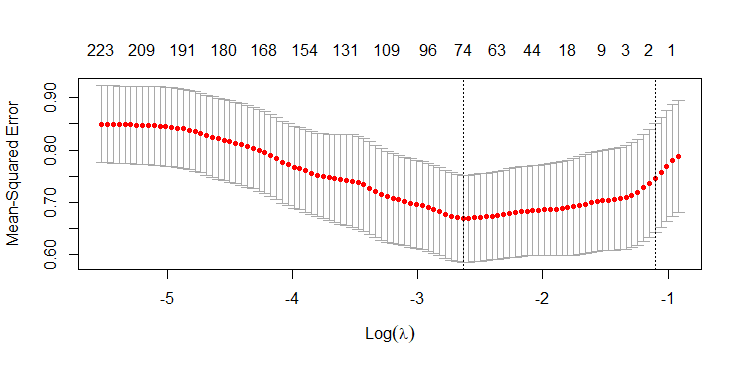
\includegraphics[width=0.8\textwidth]{lasso.png}
    \caption{Adjusting the \(\lambda\) parameter}
\end{figure}
\end{frame}
\begin{frame}
\frametitle{Lasso \& group-lasso models}
\framesubtitle{Lasso model results}
\begin{figure}[H]
    \centering
    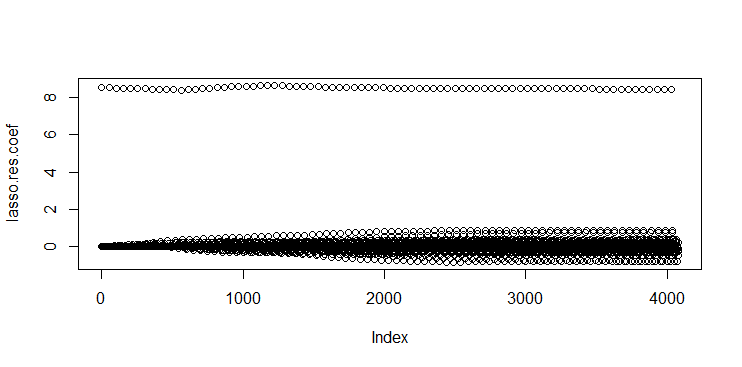
\includegraphics[width=0.8\textwidth]{lasso_result.png}
    \caption{Results of the lasso model}
\end{figure}
\end{frame}
\begin{frame}
\frametitle{Lasso \& group-lasso models}
\framesubtitle{Group-lasso model}
\begin{exampleblock}{Used data set}
Same as the lasso model, but with the grouped genes. Groups were made with the \(K\)-means
algorithm, with \num{50} groups.
\end{exampleblock}
\begin{figure}
    \centering
    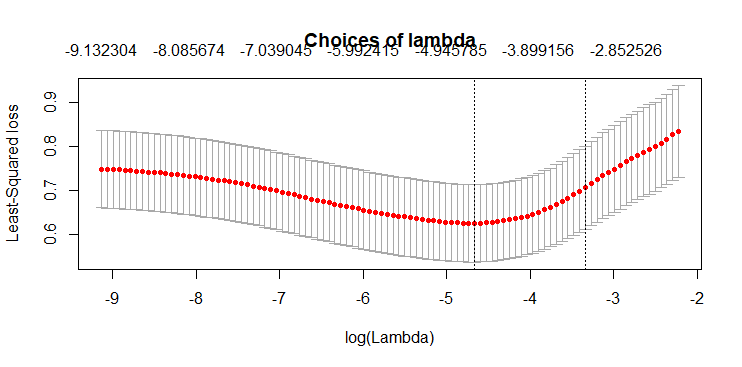
\includegraphics[width=0.8\textwidth]{glasso_l.png}
    \caption{Adjusting the \(\lambda\) parameter}
\end{figure}
\end{frame}
\begin{frame}
\frametitle{Lasso \& group-lasso models}
\framesubtitle{Group-lasso model results}
\begin{figure}[H]
    \centering
    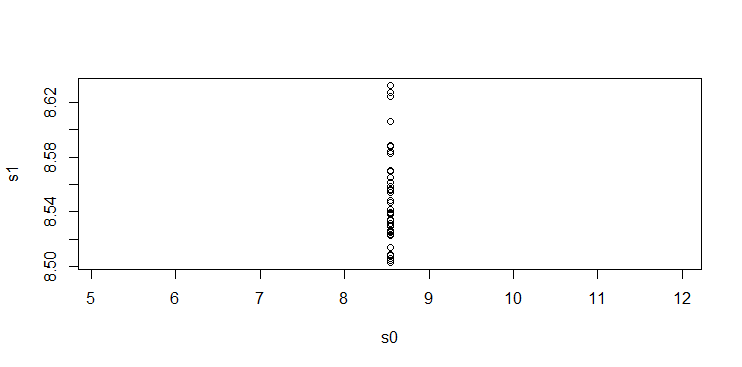
\includegraphics[width=0.8\textwidth]{group_lasso.png}
    \caption{Results of the group-lasso model}
\end{figure}
\end{frame}
\begin{frame}
\frametitle{Lasso \& group-lasso models}
\framesubtitle{Conclusions}
\begin{itemize}
    \item Lasso model is not a good idea, because it doesn't take into account the correlation between the genes.
    \item Group-lasso model is better, but still not good enough.
    \item We can't predict the phenotype of a rice with these models.
\end{itemize}
\end{frame}
\end{document}